\chapter{Implementacija i korisničko sučelje}
		
		
		\section{Korištene tehnologije i alati}
			 
			 \par
			 Komunikacija u timu realizirana je korištenjem aplikacija \underline{WhatsApp}\footnote{\url{https://www.whatsapp.com/}} i \underline{Discord}\footnote{\url{https://discord.com/}}. Za izradu UML dijagrama korišten je alat \underline{Visual Paradigm Online}\footnote{\url{https://online.visual-paradigm.com/}}. Kao sustav za upravljanje izvornim kodom korišten je \underline{Git}\footnote{\url{https://git-scm.com/}} te je udaljeni repozitorij projekta dostupan na platformi \underline{GitLab}\footnote{\url{https://gitlab.com/}}. Za izradu dokumentacije korišten je softverski sustav za pripremu dokumenata \underline{LaTeX}\footnote{\url{https://www.latex-project.org/}}.
			 \par
			 Kao razvojno okruženje korišteno je integrirano razvojno okruženje Microsofta - \underline{Microsoft Visual Studio}\footnote{\url{https://visualstudio.microsoft.com/}}. Čini ga opsežan skup alata za izgradnju ASP.NET aplikacija, desktop aplikacija i mobilnih aplikacija. Kao urednik izvornog koda za rad na \textit{frontendu} korišten je i Microsoftov uređivač izvornog koda - \underline{Visual Studio Code}\footnote{\url{https://code.visualstudio.com/}}.
			 \par
			 Za izradu \textit{frontend} dijela aplikacije korišten je \underline{.NET Framework}\footnote{\url{https://dotnet.microsoft.com}} te \underline{C sharp}\footnote{\url{https://https://docs.microsoft.com/en-us/dotnet/csharp/}}, dok je \textit{backend} dio aplikacije napravljen koristeći \underline{React}\footnote{\url{https://https://reactjs.org/}} i \underline{JavaScript}\footnote{\url{https://https://www.javascript.com/}}. .Net Framework jest radni okvir razvijen od strane Microsofta koji programerima uvelike pomaže u prevođenju i izvođenju programa. React je besplatna JavaScript biblioteka otvorenog koda za izgradnju korisničkih sučelja.
			 \par
			 Baza podataka nalazi se na poslužitelju u oblaku \underline{Microsoft Azureu}\footnote{\url{https://portal.azure.com/}}. To je računalna platforma koja omogućuje pristup i upravljanje aplikacijama i uslugama. 
			
			\eject 
		
	
		\section{Ispitivanje programskog rješenja}
			
			\subsection{Ispitivanje komponenti}
			

			
			\par
			Svi unit testovi izvršeni su automatski. Ispitivanje je provedeno po serviceima te su se tako provjeravale pojedine komponente sustava. U svakom su testu na početku dohvaćeni DbContext i Mapper.
		
			
			\noindent \textbf{Ispitni slučaj 1: Dohvaćanje svih korisnika}
			
			\noindent \textbf{Ulaz:}
			
			\begin{packed_enum}
				
				\item Stvaranje novog UserServicea
				\item Dohvaćanje metode GetAllUsers
				
			\end{packed_enum}
		
			\noindent \textbf{Očekivani izlaz:}
		
			\begin{packed_enum}
			
				\item Stvara se novi UserService
				\item Dohvaćaju se svi korisnici
				\item Rezultat testa je ispravan
			
			\end{packed_enum}
		
			\noindent \textbf{Izlaz:} Test je zadovoljen. Aplikacija je prošla test.
			
			\begin{figure}[H] 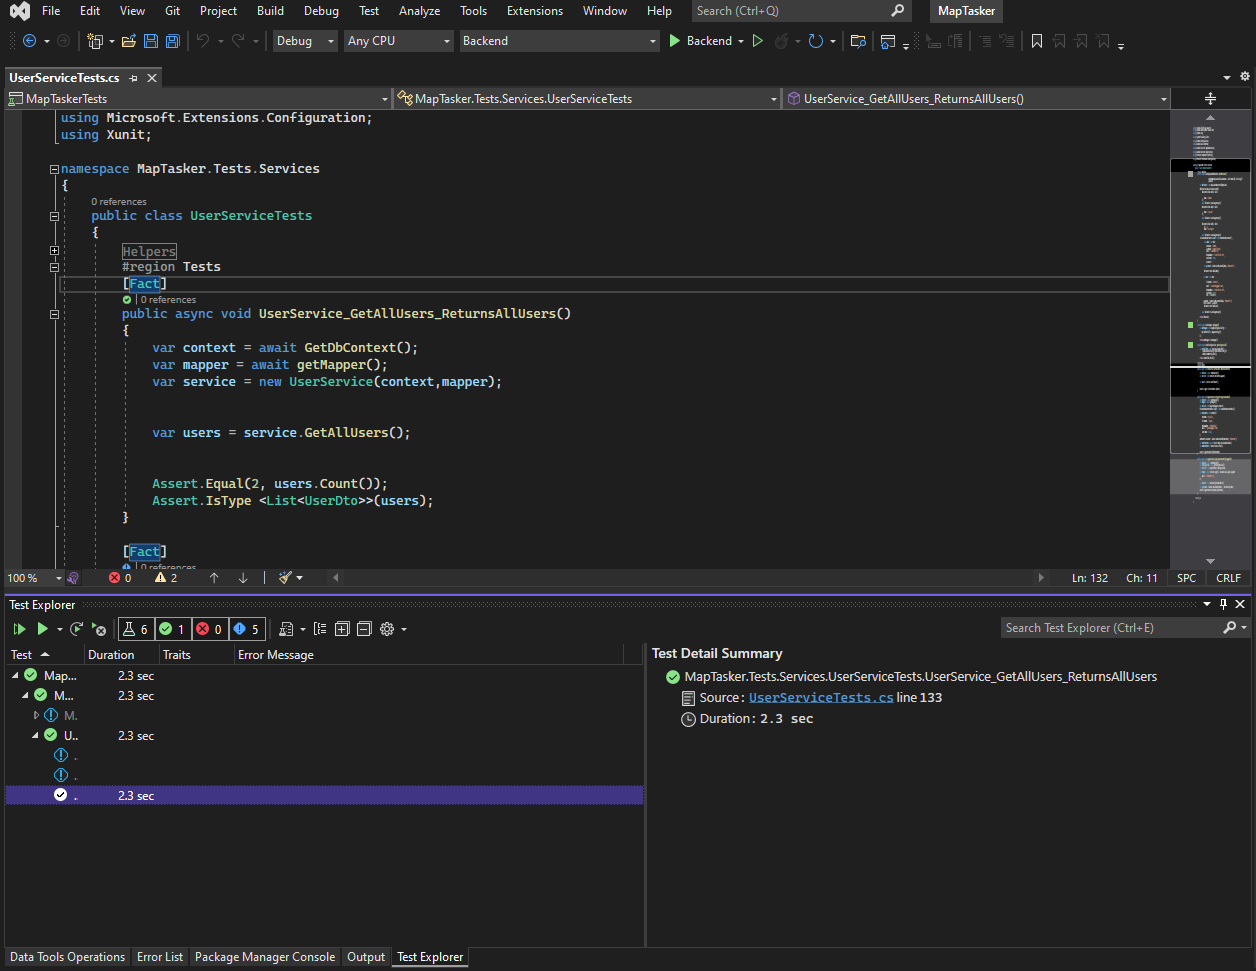
\includegraphics[width=\linewidth]{./slike/Testovi/Unit/UnitTest_1.png}
				\caption{GetAllUsers - ReturnsAllUsers Test}
			\end{figure}
			
			\eject
			
			\noindent \textbf{Ispitni slučaj 2: Uspješna registracija korisnika}
			
			\noindent \textbf{Ulaz:}
			
			\begin{packed_enum}
				
				\item Stvaranje novog RegisterServicea
				\item Kreiranje password hashera
				\item Instanciranje novog korisnika
				\item Postavljanje lozinke korisniku
				\item Dohvaćanje DTO-a Usera i ukupnog broja korisnika za provjeru
				
			\end{packed_enum}
			
			\noindent \textbf{Očekivani izlaz:}
			
			\begin{packed_enum}
				
				\item Stvara se novi RegisterService
				\item Kreira se novi password hasher
				\item Novi korisnik se uspješno stvara
				\item Lozinka se uspješno postavlja korisniku
				\item Rezultat testa je ispravan
				
			\end{packed_enum}
			
			\noindent \textbf{Izlaz:} Test je zadovoljen. Aplikacija je prošla test.
			
			\begin{figure}[H] 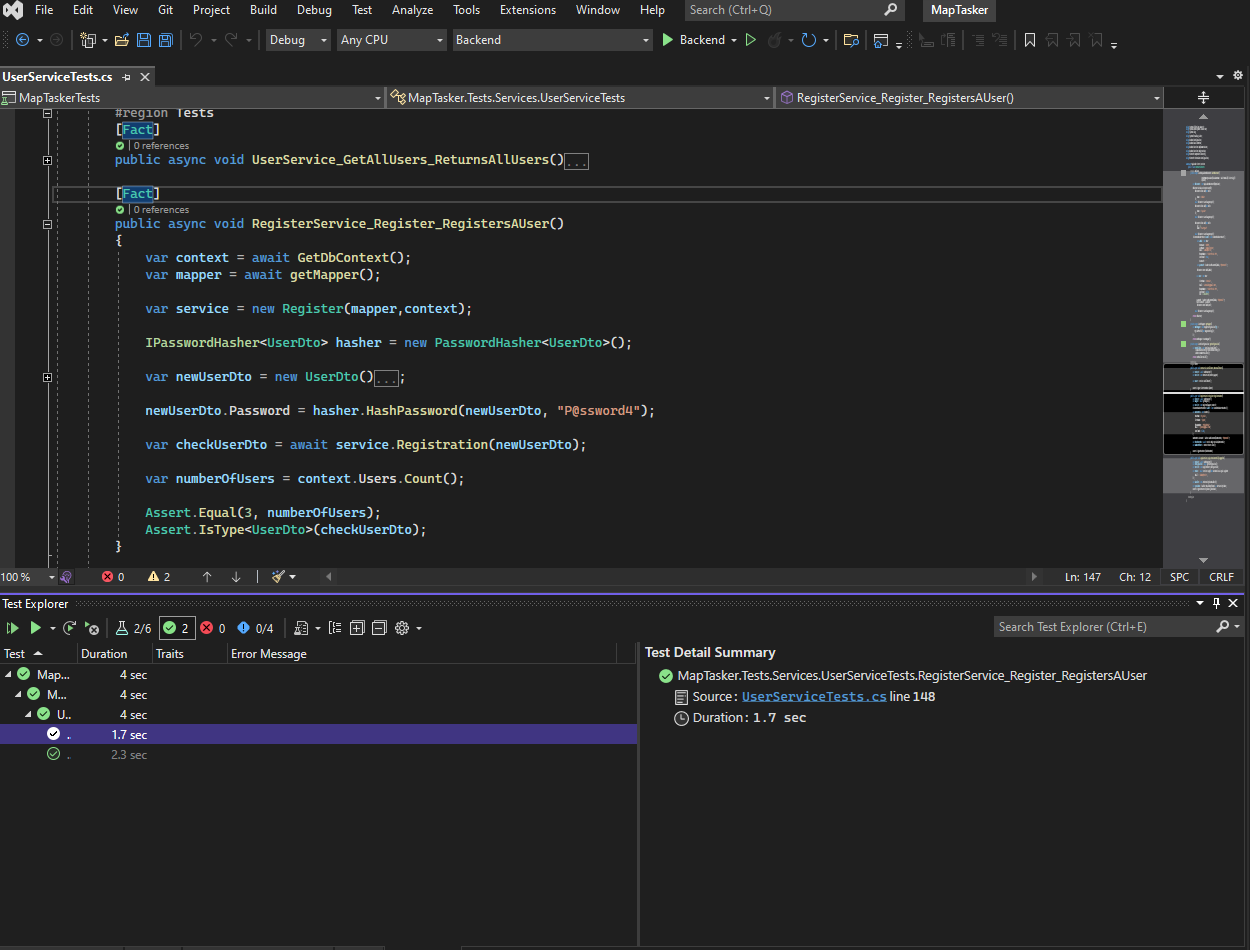
\includegraphics[width=\linewidth]{./slike/Testovi/Unit/UnitTest_2.png}
				\caption{Register - RegistersAnUser Test}
			\end{figure}
			
			\eject
		
			\noindent \textbf{Ispitni slučaj 3: Uspješna prijava korisnika}
			
			\noindent \textbf{Ulaz:}
			
			\begin{packed_enum}
				
				\item Stvaranje novog LoginServicea
				\item Kreiranje tokena koji se sastoji od e-mail adrese i lozinke
				\item Kreiranje handlera koji upravlja tokenima
				\item Dohvaćanje tokena
				
			\end{packed_enum}
			
			\noindent \textbf{Očekivani izlaz:}
			
			\begin{packed_enum}
				
				\item Stvara se novi LoginService
				\item Kreira se token za provjeru
				\item Kreira se handler koji upravlja tokenima
				\item Token se uspješno dohvaća
				\item Rezultat testa je ispravan
				
			\end{packed_enum}
			
			\noindent \textbf{Izlaz:} Test je zadovoljen. Aplikacija je prošla test.
			
			\begin{figure}[H] 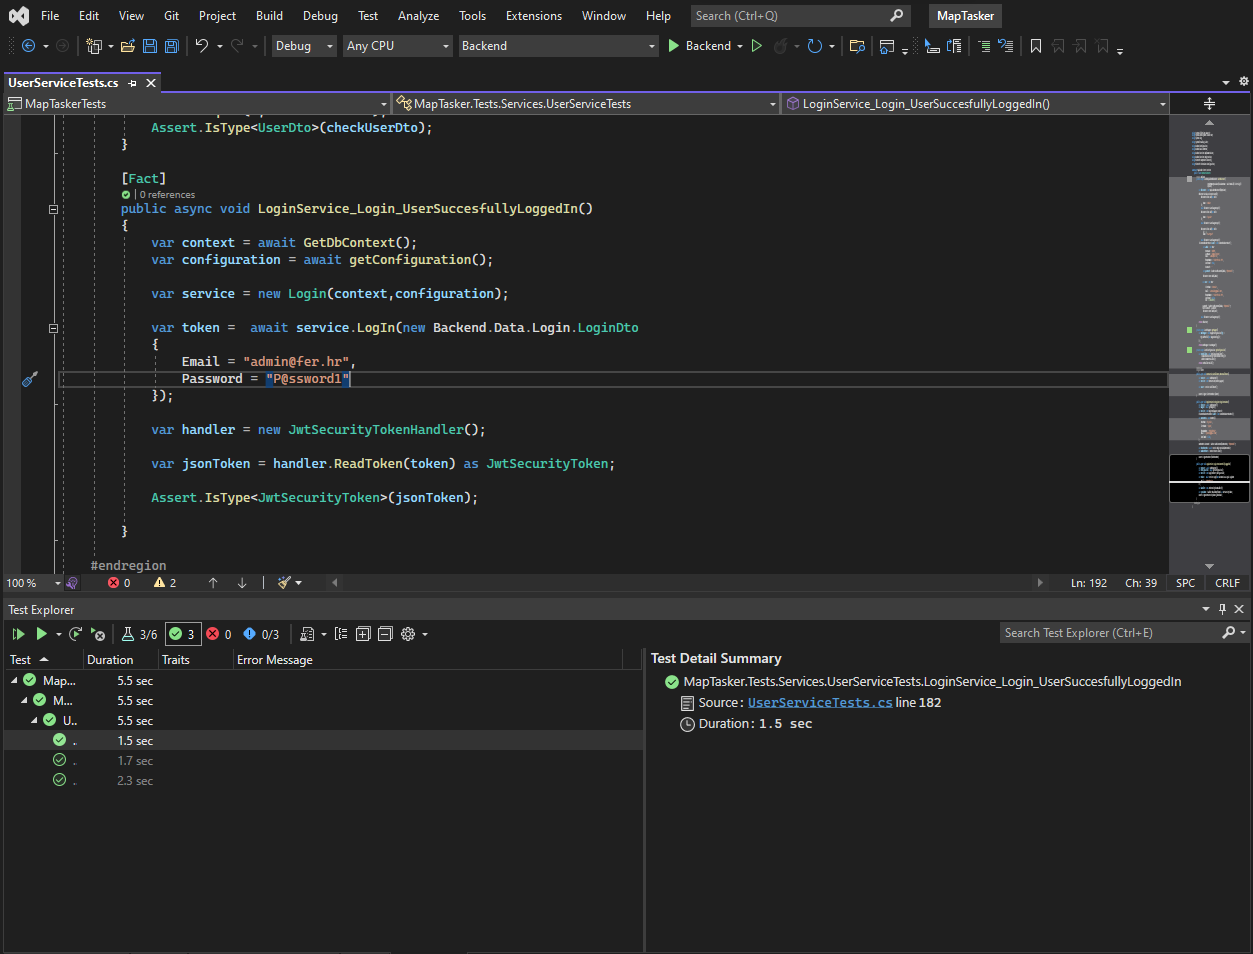
\includegraphics[width=\linewidth]{./slike/Testovi/Unit/UnitTest_3.png}
				\caption{UserSuccesfullyLoggedIn Test}
			\end{figure}
			
			\eject
			
			\noindent \textbf{Ispitni slučaj 4: Dohvaćanje svih prijava nestanka}
			
			\noindent \textbf{Ulaz:}
			
			\begin{packed_enum}
				
				\item Stvaranje novog generatora Id-a
				\item Kreiranje novog MissingReport Servicea
				\item Dohvaćanje svih prijava nestanaka metodom GetAllMissingReports
				
			\end{packed_enum}
			
			\noindent \textbf{Očekivani izlaz:}
			
			\begin{packed_enum}
				
				\item Stvara se generator Id-a
				\item Uspješno kreiranje MissingReporta
				\item Uspješno se dohvaćaju sve prijave nestanaka
				\item Rezultat testa je ispravan
				
			\end{packed_enum}
			
			\noindent \textbf{Izlaz:} Test je zadovoljen. Aplikacija je prošla test.
			
			\begin{figure}[H] 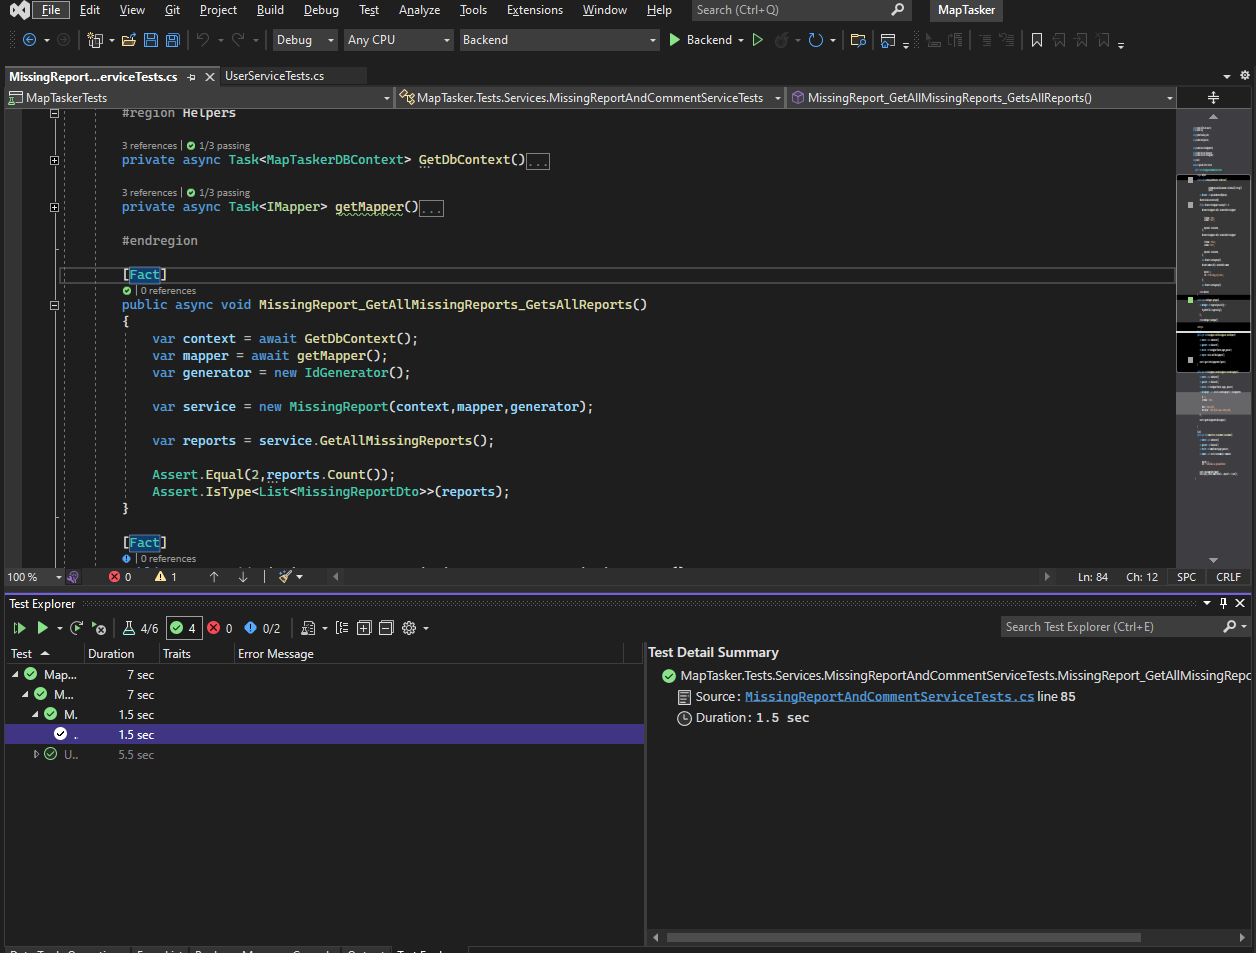
\includegraphics[width=\linewidth]{./slike/Testovi/Unit/UnitTest_4.png}
				\caption{GetAllMissingReports Test}
			\end{figure}
			
			\eject
			
			\noindent \textbf{Ispitni slučaj 5: Stvaranje prijave nestanka}
			
			\noindent \textbf{Ulaz:}
			
			\begin{packed_enum}
				
				\item Stvaranje novog generatora Id-a
				\item Kreiranje MissingReport Servicea
				\item Instanciranje prijave nestanka
				
			\end{packed_enum}
			
			\noindent \textbf{Očekivani izlaz:}
			
			\begin{packed_enum}
				
				\item Stvara se generator Id-a
				\item Uspješno kreiranje MissingReport Servicea
				\item Prijava nestanka uspješno je instancirana
				\item Rezultat testa je ispravan
				
			\end{packed_enum}
			
			\noindent \textbf{Izlaz:} Test je zadovoljen. Aplikacija je prošla test.
			
			\begin{figure}[H] 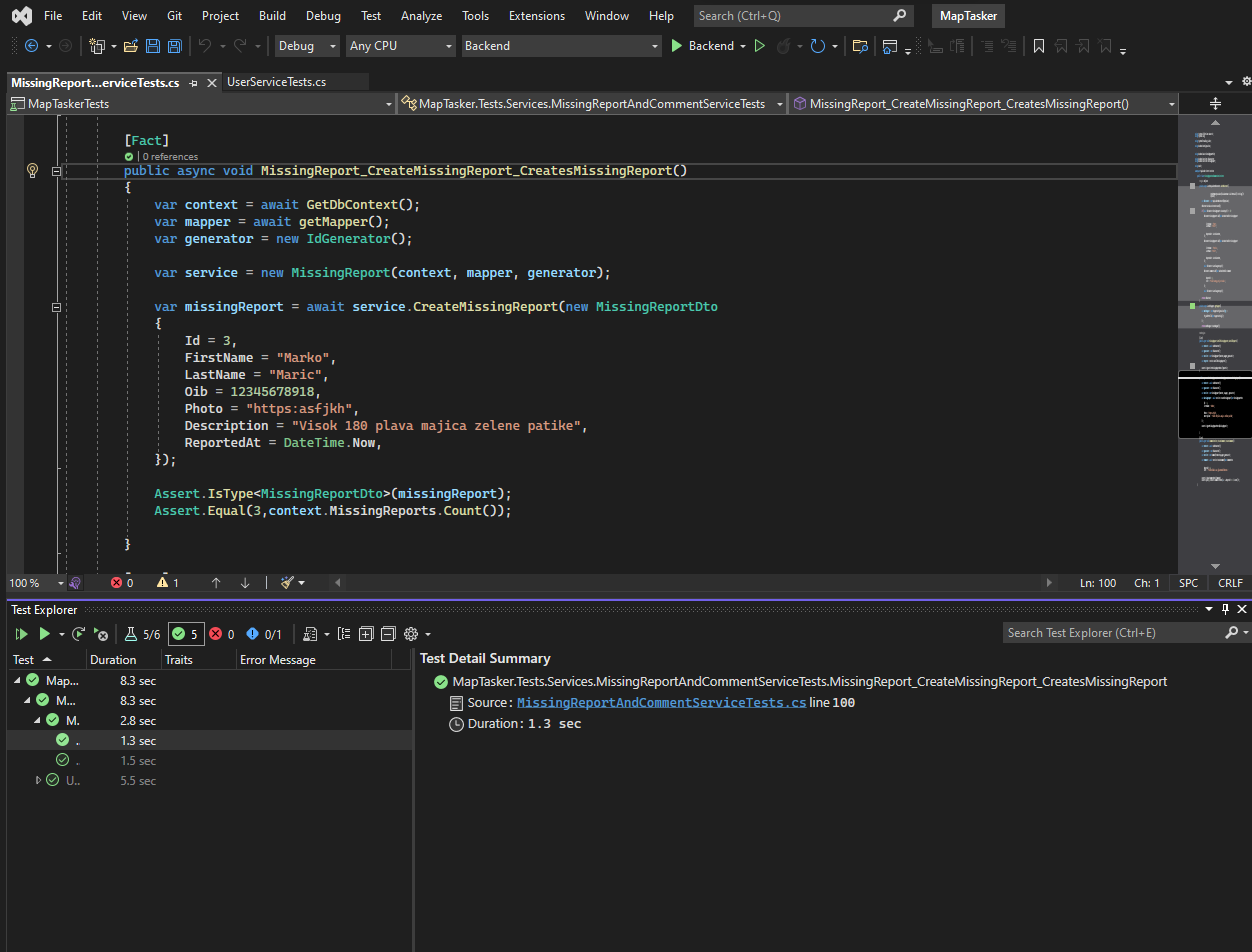
\includegraphics[width=\linewidth]{./slike/Testovi/Unit/UnitTest_5.png}
				\caption{CreatesMissingReport Test}
			\end{figure}
			
			\eject
			
			\noindent \textbf{Ispitni slučaj 6: Kreiranje komentara}
			
			\noindent \textbf{Ulaz:}
			
			\begin{packed_enum}
				
				\item Stvaranje novog generatora Id-a
				\item Kreiranje Comment Servicea
				\item Instanciranje novog komentara
				
			\end{packed_enum}
			
			\noindent \textbf{Očekivani izlaz:}
			
			\begin{packed_enum}
				
				\item Stvara se generator Id-a
				\item Uspješno se kreiran Comment Service
				\item Komentar je uspješno instanciran
				\item Rezultat testa je ispravan
				
			\end{packed_enum}
			
			\noindent \textbf{Izlaz:} Test je zadovoljen. Aplikacija je prošla test.
			
			\begin{figure}[H] 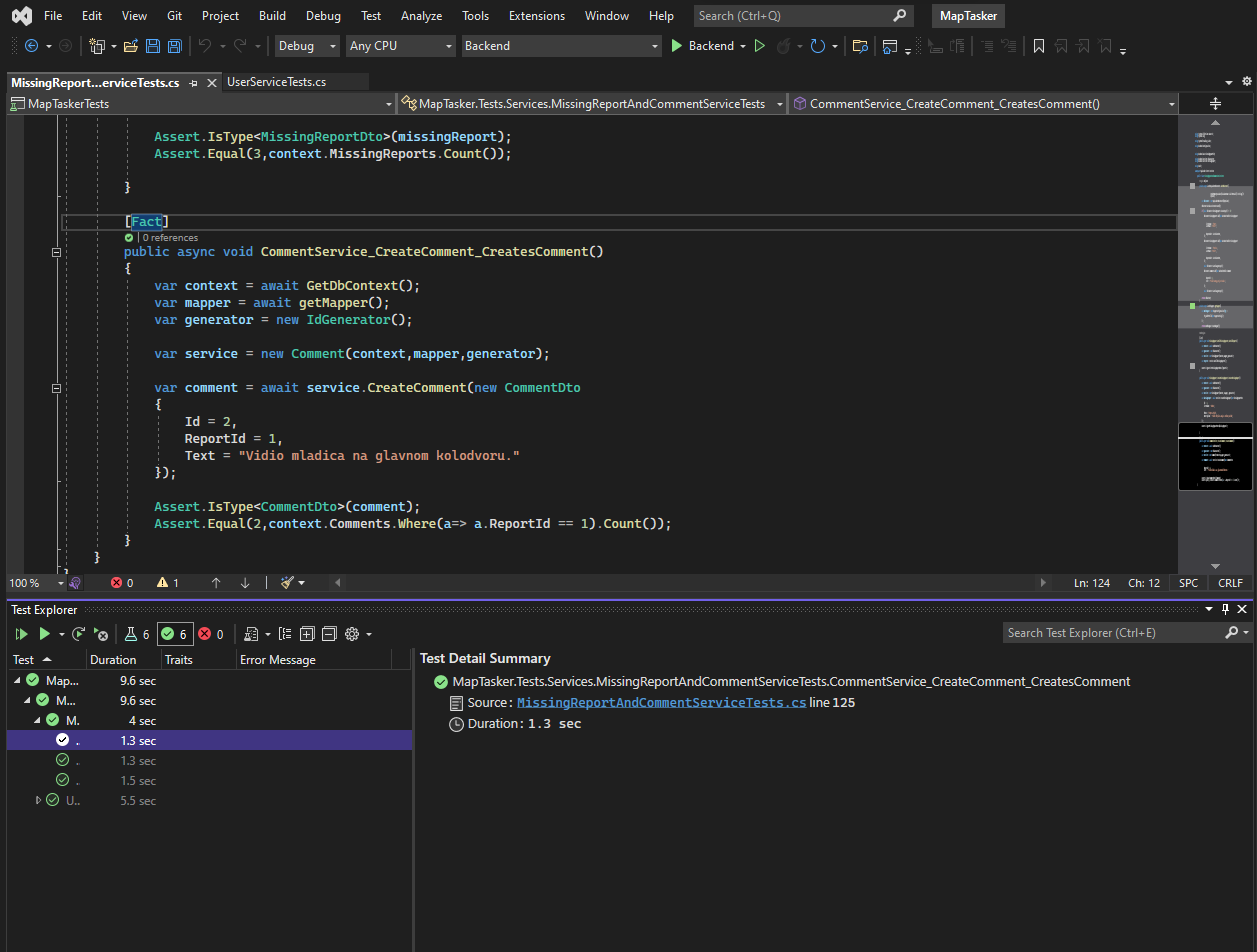
\includegraphics[width=\linewidth]{./slike/Testovi/Unit/UnitTest_6.png}
				\caption{CreatesComments Test}
			\end{figure}
			
			\eject
			
			
			
			\subsection{Ispitivanje sustava}
			
			\par
			Svi Selenium testovi izvršeni su automatski. Ispitivanje je provedeno po obrascima uporabe. Ispitani su obrasci uporabe:
			
			\begin{packed_enum}
				
				\item UC1 - Registracija u sustav
				\item UC2 - Prijava u sustav
				\item UC4 - Prijava nestale osobe
				\item UC5 - Komentiranje prijave nestale osobe
				
			\end{packed_enum}
		
			
			\noindent \textbf{Ispitni slučaj 1: Registracija}
			
			\noindent \textbf{Ulaz:}
			
			\begin{packed_enum}
				
				\item Učitavanje početne stranice i namještanje veličine prozora
				\item Pritisak na gumb "Register"
				\item Korisnik unosi tražene podatke te odabire ulogu koju želi
				
			\end{packed_enum}
			
			\noindent \textbf{Očekivani izlaz:}
			
			\begin{packed_enum}
				
				\item Početna stranica uspješno se učitava
				\item Učitavanje forme za registraciju
				\item Korisnik prima obavijest o uspješno obavljenoj registraciji
				\item Rezultat testa je ispravan
				
			\end{packed_enum}
			
			\noindent \textbf{Izlaz:} Test je zadovoljen. Aplikacija je prošla test.
			
			\begin{figure}[H] 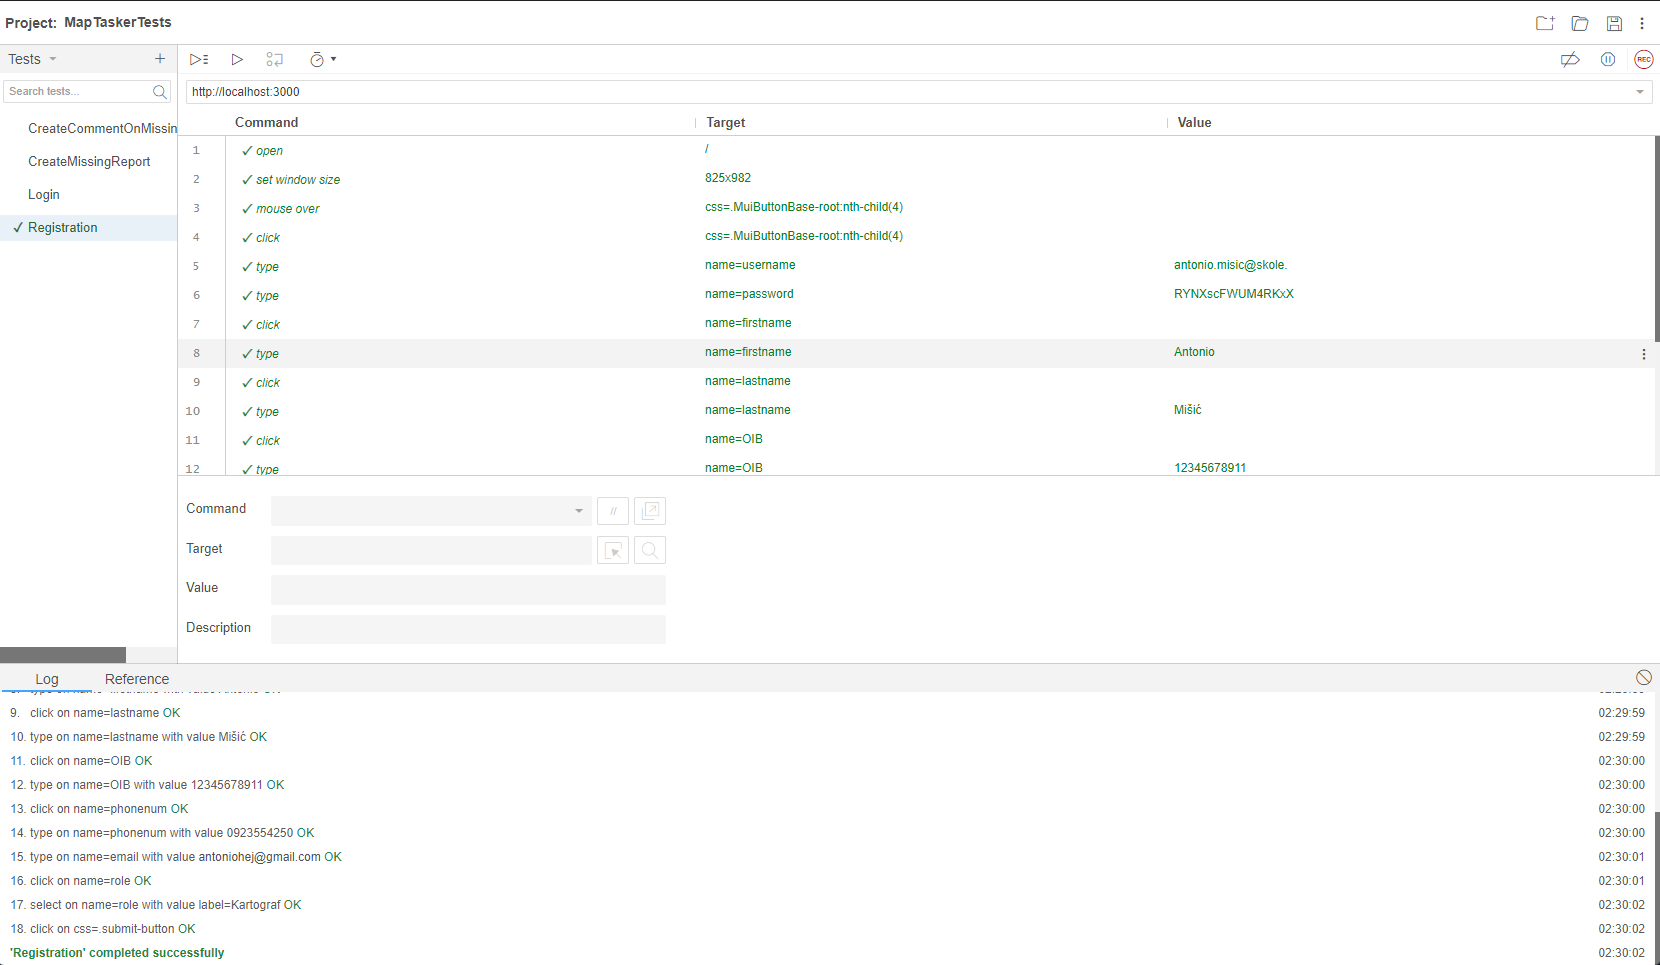
\includegraphics[width=\linewidth]{./slike/Testovi/Selenium/Selenium_1.png}
				\caption{Registration Test}
			\end{figure}
			
			\eject
			
			\noindent \textbf{Ispitni slučaj 2: Prijava}
			
			\noindent \textbf{Ulaz:}
			
			\begin{packed_enum}
				
				\item Učitavanje početne stranice i namještanje veličine prozora
				\item Pritisak na gumb "Login"
				\item Korisnik unosi e-mail adresu i lozinku
				
			\end{packed_enum}
			
			\noindent \textbf{Očekivani izlaz:}
			
			\begin{packed_enum}
				
				\item Početna stranica uspješno se učitava
				\item Učitavanje forme za prijavu
				\item Korisnik je uspješno prijavljen u sustav
				\item Rezultat testa je ispravan
				
			\end{packed_enum}
			
			\noindent \textbf{Izlaz:} Test je zadovoljen. Aplikacija je prošla test.
			
			\begin{figure}[H] 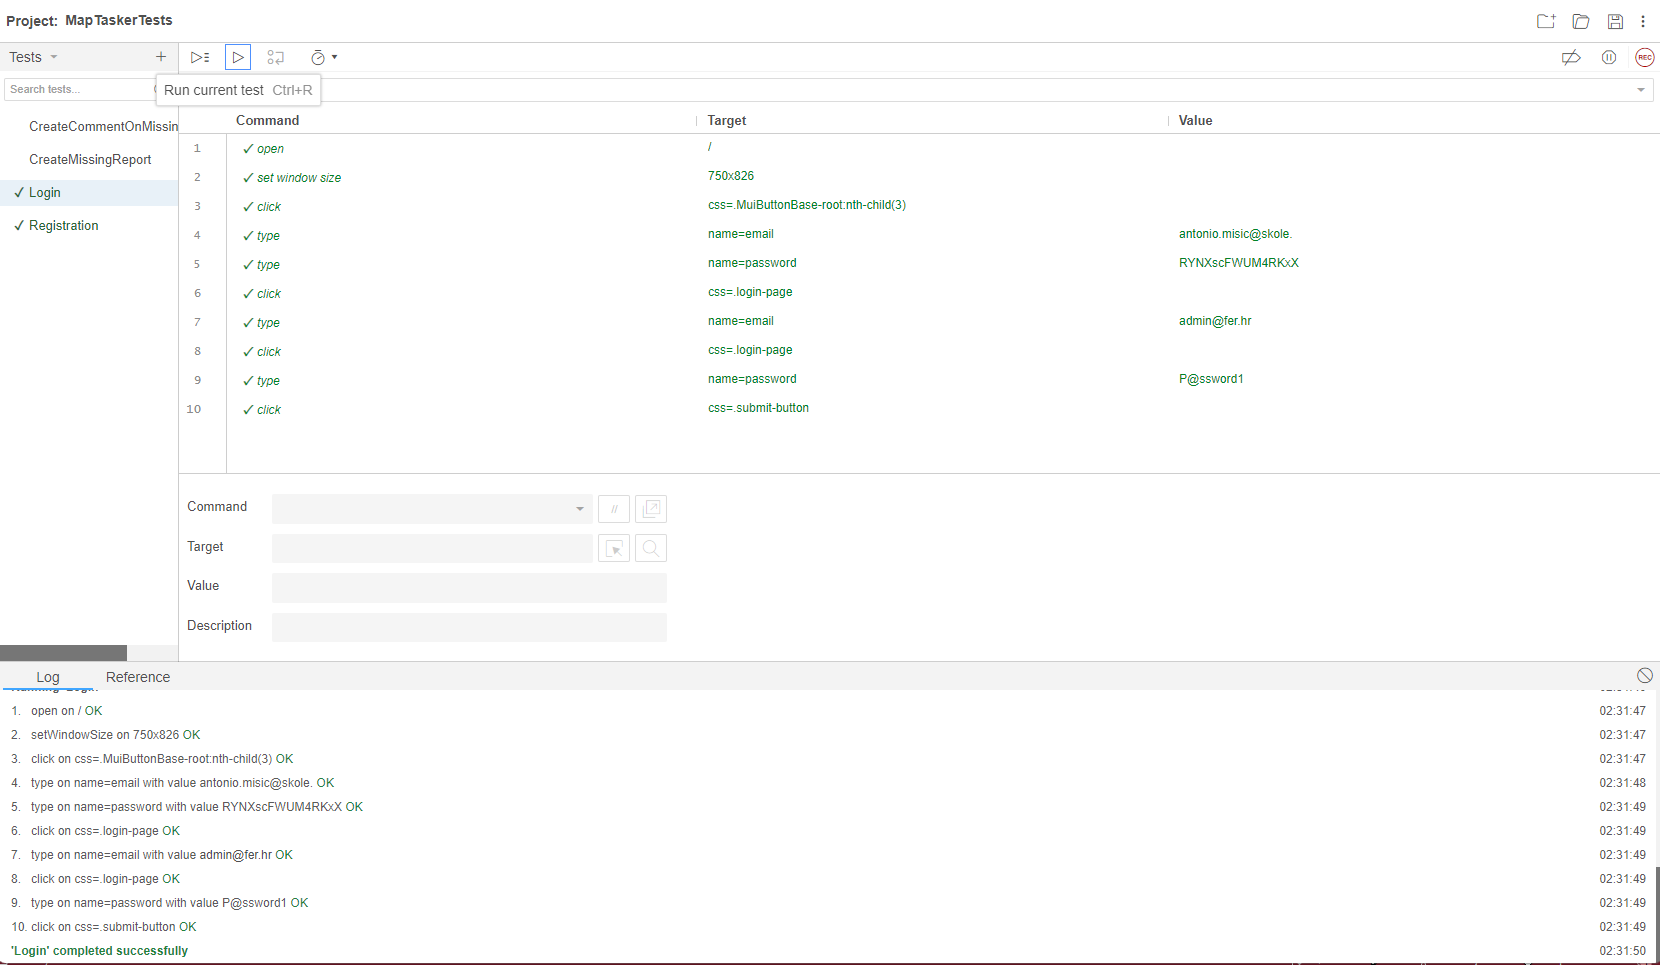
\includegraphics[width=\linewidth]{./slike/Testovi/Selenium/Selenium_2.png}
				\caption{Login Test}
			\end{figure}
			
			\eject
			
			\noindent \textbf{Ispitni slučaj 3: Kreiranje prijave nestanka}
			
			\noindent \textbf{Ulaz:}
			
			\begin{packed_enum}
				
				\item Učitavanje početne stranice i namještanje veličine prozora
				\item Pritisak na gumb "Prijavi"
				\item Unošenje podataka o nestaloj osobi
				
			\end{packed_enum}
			
			\noindent \textbf{Očekivani izlaz:}
			
			\begin{packed_enum}
				
				\item Početna stranica uspješno se učitava
				\item Učitavanje forme za prijavu nestanka osobe
				\item Obavijest o uspješnoj prijavi nestale osobe
				\item Rezultat testa je ispravan
				
			\end{packed_enum}
			
			\noindent \textbf{Izlaz:} Test je zadovoljen. Aplikacija je prošla test.
			
			\begin{figure}[H] 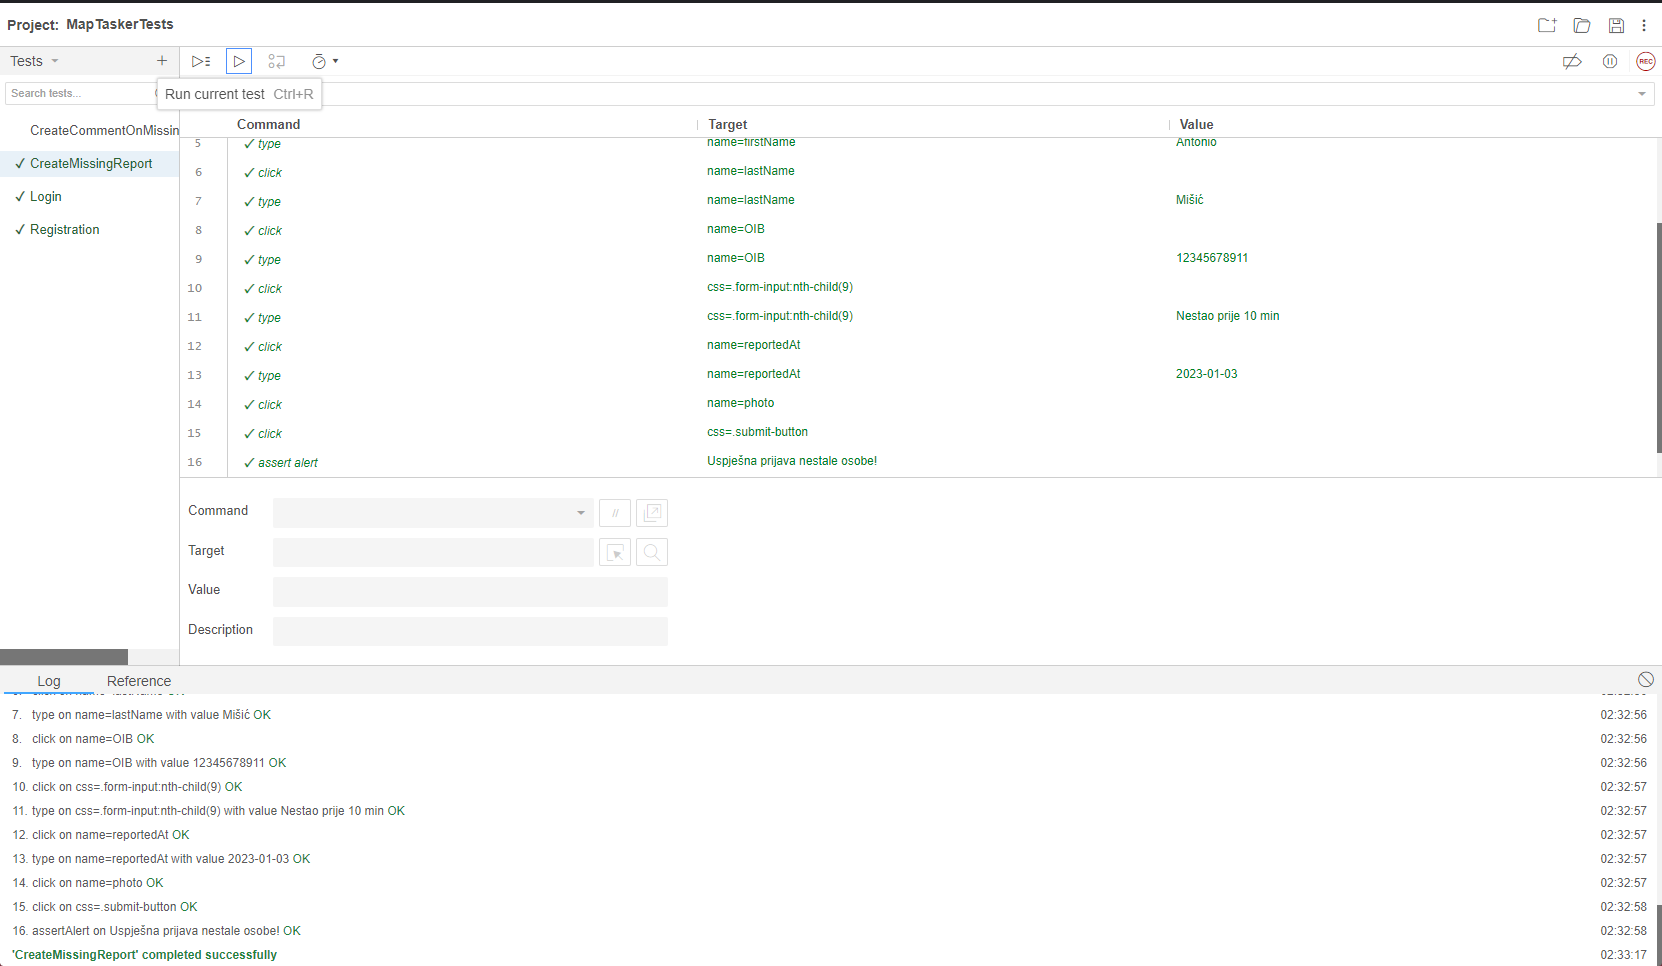
\includegraphics[width=\linewidth]{./slike/Testovi/Selenium/Selenium_3.png}
				\caption{CreateMissingReport Test}
			\end{figure}
			
			\eject
			
			\noindent \textbf{Ispitni slučaj 4: Kreiranje komentara na prijavu nestanka}
			
			\noindent \textbf{Ulaz:}
			
			\begin{packed_enum}
				
				\item Učitavanje početne stranice i namještanje veličine prozora
				\item Pritisak na gumb "Nestale osobe"
				\item Stvaranje komentara kraj nestale osobe
				
			\end{packed_enum}
			
			\noindent \textbf{Očekivani izlaz:}
			
			\begin{packed_enum}
				
				\item Početna stranica uspješno se učitava
				\item Učitavanje stranice s nestalim osobama
				\item Komentar je prikazan na stranici
				\item Rezultat testa je ispravan
				
			\end{packed_enum}
			
			\noindent \textbf{Izlaz:} Test je zadovoljen. Aplikacija je prošla test.
			
			\begin{figure}[H] 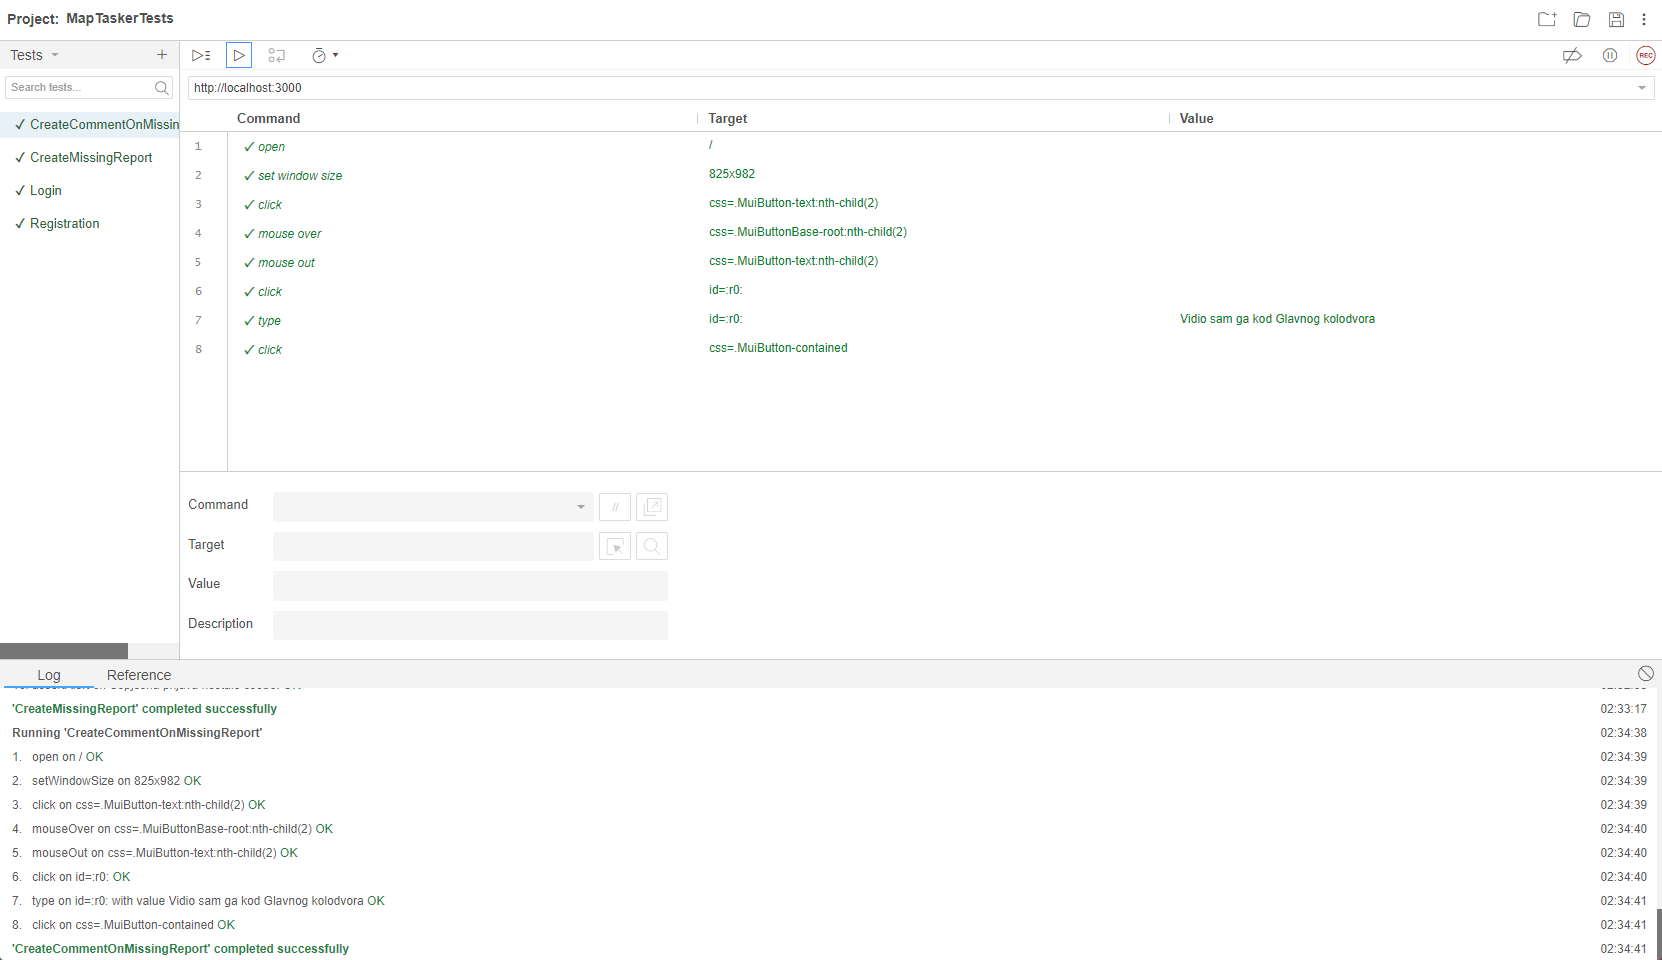
\includegraphics[width=\linewidth]{./slike/Testovi/Selenium/Selenium_4.png}
				\caption{CreateComment Test}
			\end{figure}
			
			\eject
		
		
		\section{Dijagram razmještaja}
			
			\textbf{\textit{dio 2. revizije}}
			
			 \textit{Potrebno je umetnuti \textbf{specifikacijski} dijagram razmještaja i opisati ga. Moguće je umjesto specifikacijskog dijagrama razmještaja umetnuti dijagram razmještaja instanci, pod uvjetom da taj dijagram bolje opisuje neki važniji dio sustava.}
			
			\eject 
		
		\section{Upute za puštanje u pogon}
		
			\textbf{\textit{dio 2. revizije}}\\
		
			 \textit{U ovom poglavlju potrebno je dati upute za puštanje u pogon (engl. deployment) ostvarene aplikacije. Na primjer, za web aplikacije, opisati postupak kojim se od izvornog kôda dolazi do potpuno postavljene baze podataka i poslužitelja koji odgovara na upite korisnika. Za mobilnu aplikaciju, postupak kojim se aplikacija izgradi, te postavi na neku od trgovina. Za stolnu (engl. desktop) aplikaciju, postupak kojim se aplikacija instalira na računalo. Ukoliko mobilne i stolne aplikacije komuniciraju s poslužiteljem i/ili bazom podataka, opisati i postupak njihovog postavljanja. Pri izradi uputa preporučuje se \textbf{naglasiti korake instalacije uporabom natuknica} te koristiti što je više moguće \textbf{slike ekrana} (engl. screenshots) kako bi upute bile jasne i jednostavne za slijediti.}
			
			
			 \textit{Dovršenu aplikaciju potrebno je pokrenuti na javno dostupnom poslužitelju. Studentima se preporuča korištenje neke od sljedećih besplatnih usluga: \href{https://aws.amazon.com/}{Amazon AWS}, \href{https://azure.microsoft.com/en-us/}{Microsoft Azure} ili \href{https://www.heroku.com/}{Heroku}. Mobilne aplikacije trebaju biti objavljene na F-Droid, Google Play ili Amazon App trgovini.}
			
			
			\eject 

